\section{Graded Assignment 2}\label{sec:graded_assignment_2}

% A full answer and result analysis is expected for task 3 and 4. For task 3 you should include a plot of the different states over time as well as the error states for your choice of parameters, in addition to NEES and NIS over time for the same set of parameters. In task 4 the same plots are expected, of course excluding anything that needs the ground truth. For both tasks it should be made clear why the parameters were chosen in terms of error metrics, consistency and overall result. Answers and analysis should connect theory and results to the real world, and show your understanding for the problem and solution. Try to connect the reuslts on the simulated data to the results of the real data where it is possible. 

An error-state Kalman filter (ESKF) for a GNSS-aided fixed-wing UAV was implemented in MATLAB. The implementation is based on the standard formulation in \cite{Sola}. But most notably, IMU sensor correction matrices has been added to counteract any mounting errors, scaling errors and orthogonality errors in the accelerometer and rate gyro. Furthermore, leverarm componsation for the GNSS receiver is also implemented.

\subsection{INS for simulated fixed-wing UAV}

%Tuning values, how we tuned (NIS, NEES, RMSE, want bias to converge somewhat, not wander, commen sense)

%Heading observability - heading error large, spikes?? Probably low when turning, then larger when straight/no acceleration. Also see this in attitude NEES compared to others.

%Misalignment matrix

% discuss bias models

The ESKF was first tuned to a simulated dataset. The GNSS measurement standard deviation was tuned to $0.4$ in each degree of freedom. The measurement noise covariance is therefore $R=0.16 I ^2$. For the accelerometer the measurement noise covariance and bias driving noise covariance was tuned to be $q_{a} = (\SI{4e-2})^2$ and $ q_{ab} = (\SI{1e-3})^2$ respectively. Similarily for the rate gyro the measurement noise covariance and bias driving noise covariance was tuned to be $q_{\omega} = (\SI{8e-4})^2$ and $q_{\omega b} = (\SI{1e-6})^2$ respectively. Finally the time constants in the Gauss-Markov bias processes were both tuned to be $T_b = \SI{1e8}{s}$.

Firstly, the tuning was based on common sense. For instance the GNSS measurement covariance was initially based on a reasonable guess from a physical perspective and then more thoroughly tuned. This more thorough tuning was based on calculating and plotting the errors in position, velocity, attitude and bias. Furthermore the corresponding NEES in position, velocity, attitude and biases, as well as the overall NEES and NIS was calculated and analysed during the tuning process. 

The resulting position estimate is plotted in \cref{fig:ga_2_sim_trajectory}, the state and state errors are presented in \cref{fig:ga_2_sim_state} and \cref{fig:ga_2_sim_errors} and finally the consistency analysis is presented in \cref{fig:ga_2_sim_consistency}. Note that the consistency figures are presented in logarithmic scale.

\begin{figure}[ht]
    \centering
	\begin{subfigure}[b]{0.45\textwidth}
		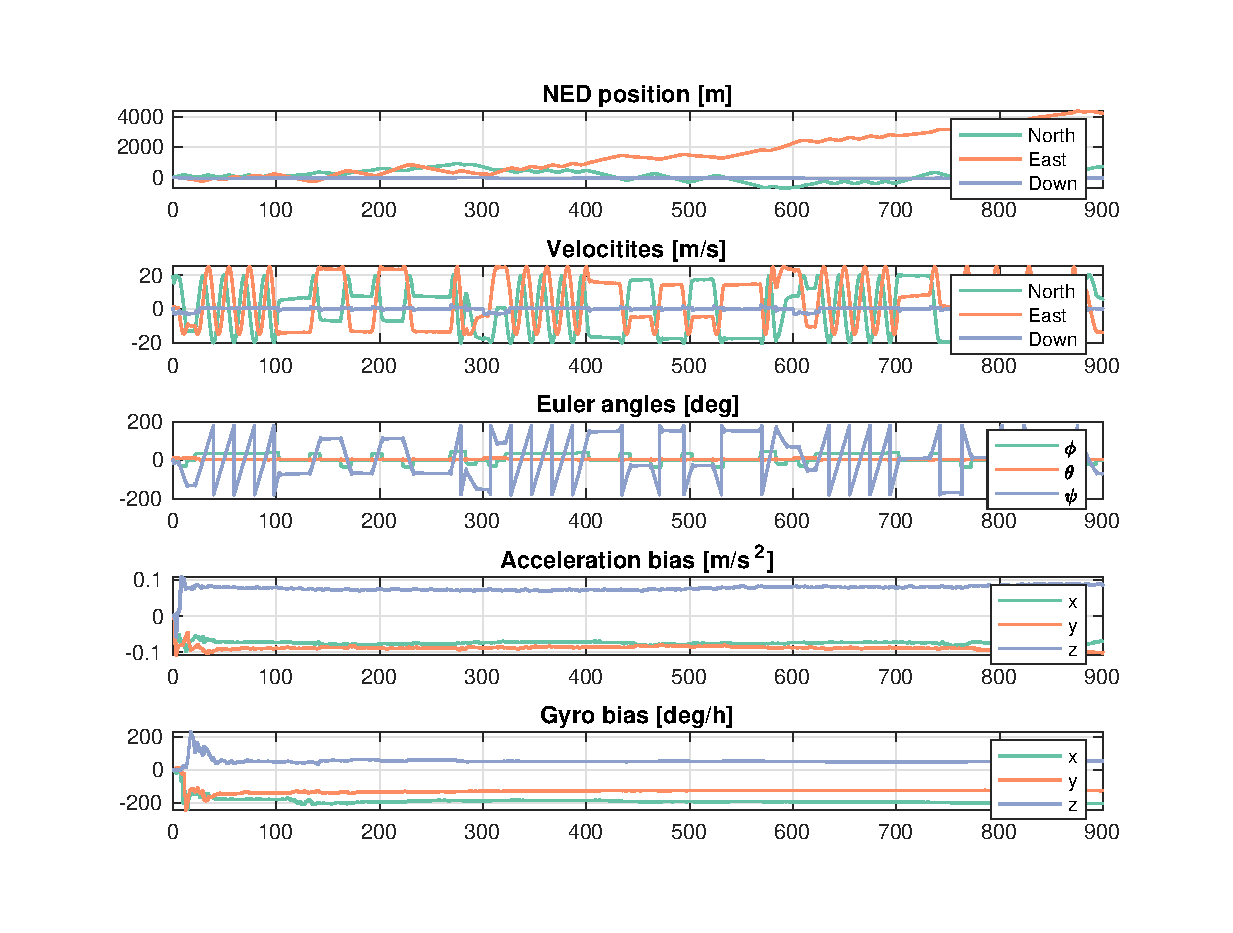
\includegraphics[width=\textwidth]{figures/ga_2/sim_state}
		\caption{UAV states}
		\label{fig:ga_2_sim_state}
	\end{subfigure}%
       ~
	\begin{subfigure}[b]{0.45\textwidth}
		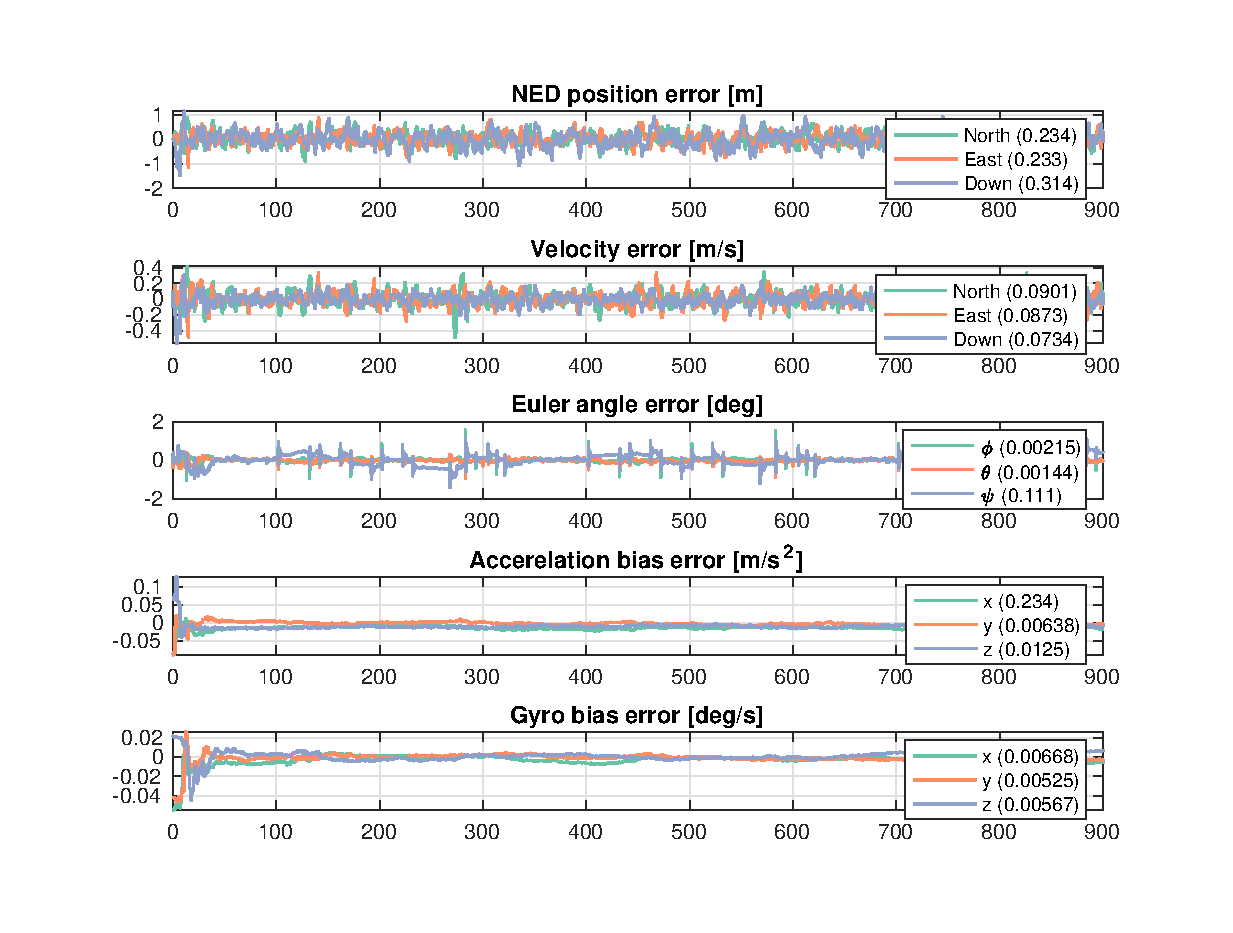
\includegraphics[width=\textwidth]{figures/ga_2/sim_errors}
		\caption{UAV state errors}
		\label{fig:ga_2_sim_errors}
	\end{subfigure}
    \label{fig:ga_2_sim_state_errors} 
\end{figure}

\begin{figure}[ht]
    \centering
	\begin{subfigure}[b]{0.45\textwidth}
		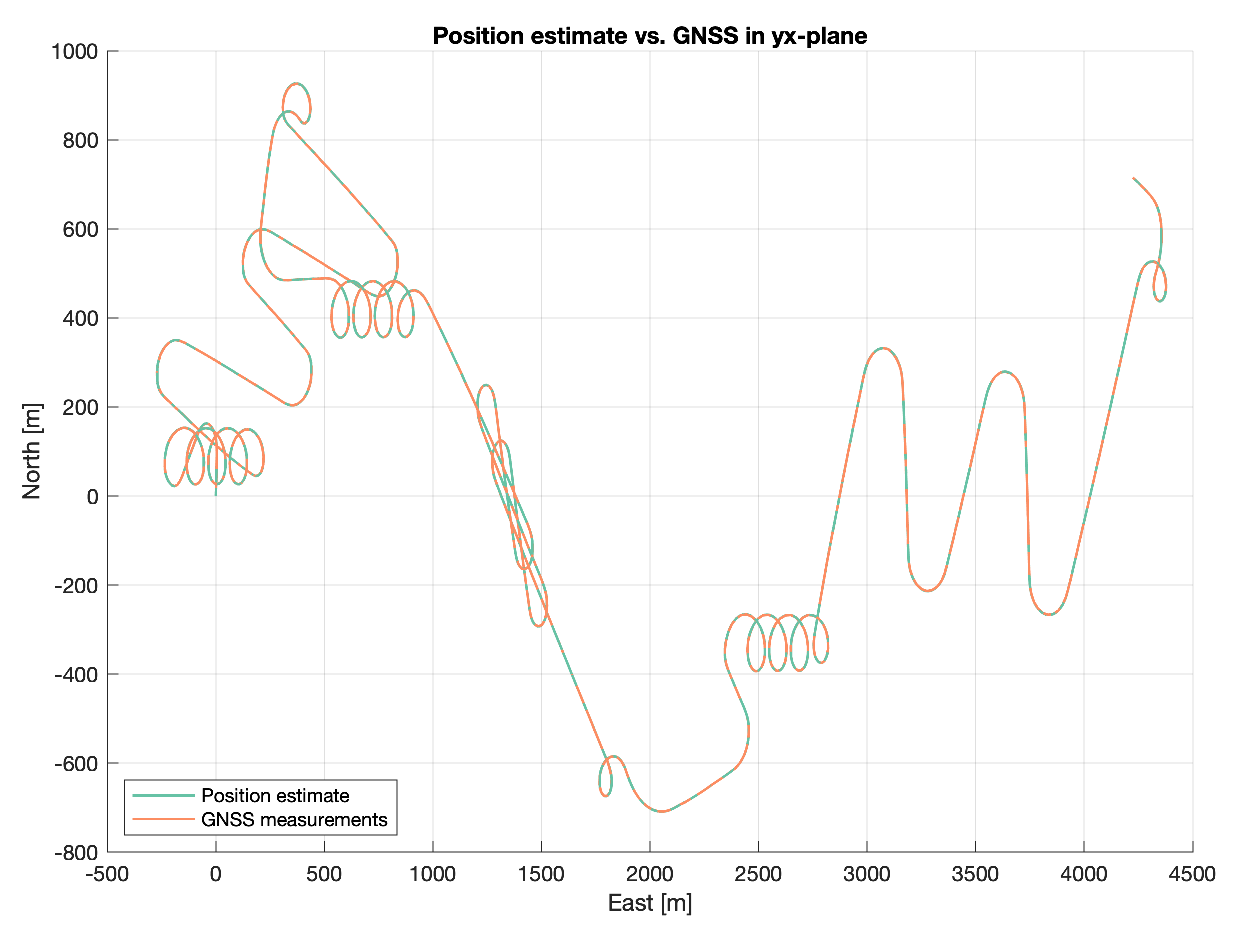
\includegraphics[width=\textwidth]{figures/ga_2/sim_trajectory.eps}
    \caption{Estimated UAV trajectory}
    \label{fig:ga_2_sim_trajectory}
	\end{subfigure}%
       ~
	\begin{subfigure}[b]{0.45\textwidth}
		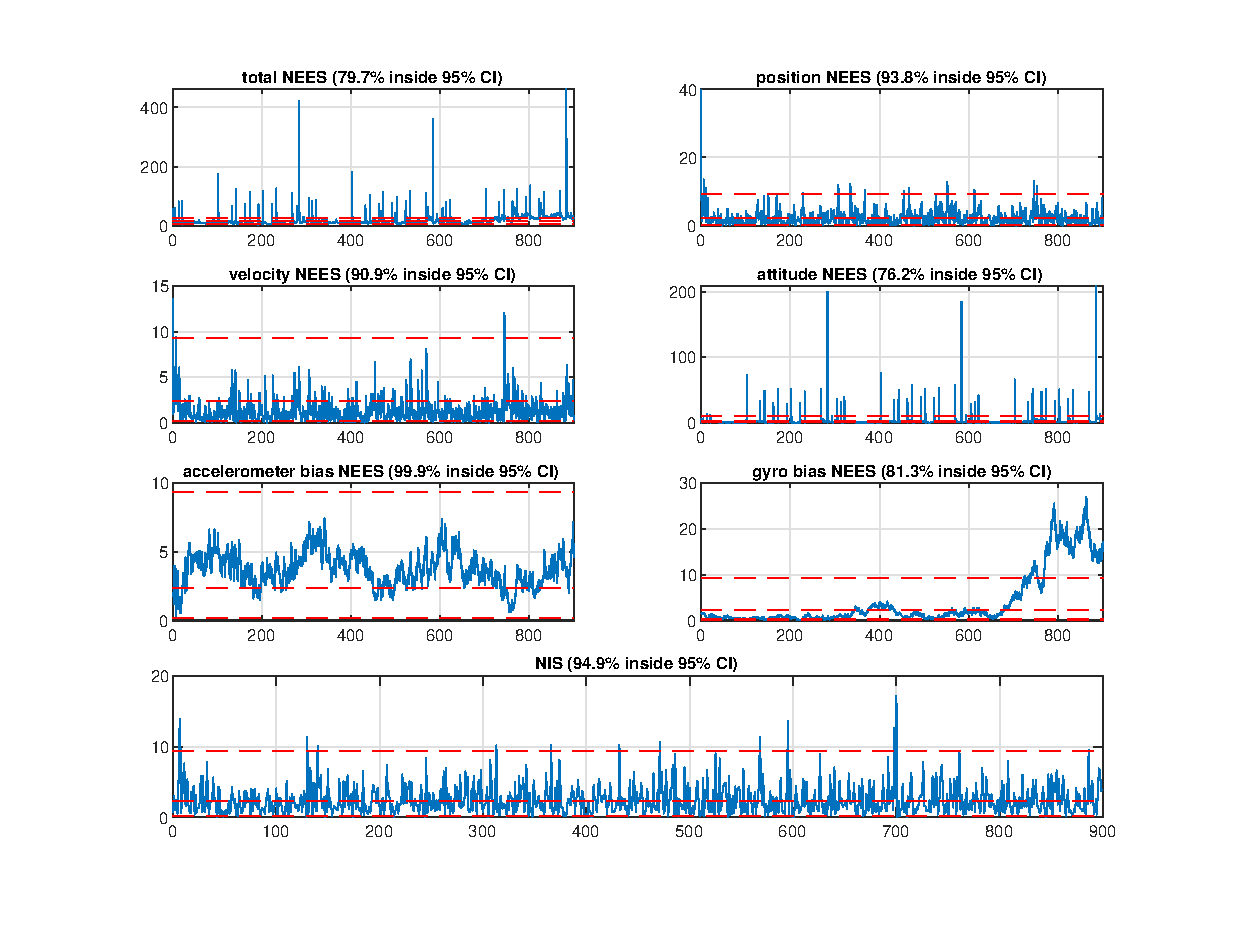
\includegraphics[width=\textwidth]{figures/ga_2/sim_consistency.eps}
    \caption{UAV consistency analysis}
    \label{fig:ga_2_sim_consistency}
	\end{subfigure}
    \label{fig:ga_2_sim_trajectory_consistency} 
\end{figure}

The ESKF was in particular tuned such that the bias states converged nicely, such that the errors propagated in the system from sensor drift were minimised. It should be emphasised that one of the main features that makes the ESKF robust is the IMU bias estimation, and it was therefore also emphasised in the tuning process.

The consistency was also emphasised when tuning the ESKF. We see from \cref{fig:ga_2_sim_consistency} that most of the different normalized square errors are all in the 80\% or 90\% range inside the calculated confidence intervals, which was found to be satisfactory. One should especially note that the attitude NEES is only about 76\% inside the confidence interval. Studying the heading error in \cref{fig:ga_2_sim_errors} can give some insight into why this might be the lowest NEES. It is observed that the heading is at certain time intervals far off the ground truth, which is also confirmed by the RMSE of 0.111. This is about two magnitudes higher error than for pitch and roll. This is caused by the fact that pitch and roll are directly observable from the gravitational force acting on the accelerometer. Heading, on the other hand, is only observable when the system is exited by a manoeuvre. The heading error, therefore, has certain sections where it is unobservable and the update step is not able to correct the constant offset from the true value. This is further supported by studying the time intervals when the UAV is doing a spiral manoeuvre e.g. from about 300 to 400 seconds or from 600 to 700 seconds. In these intervals the heading is observable and as a consequence, we observe that the error drops to the same magnitude as the pitch and roll, before it starts acting unexpectedly again when the UAV starts flying straight. This issue might be why both the attitude NEES and total NEES is somewhat worse than the others. So the heading estimation would therefore not work if the UAV was standing still. 

When letting the sensor correction matrices be identity matrices, and thereby removing any sensor correction, the ESKF estimation performance is noticeably worse. While the filter is still able to reliably estimative velocity and position with the aid of the GNSS, the estimates of heading and sensor biases are much worse. Most importantly, the rate gyro and accelerometer biases no longer converge to the true sensor biases. This means we are not able to remove the bias in the measurements, and as a consequence, they are integrated and propagated through the Kalman filter. This makes all the RMSEs significantly worse, and especially the heading now drifts quickly when the UAV is not turning.

Then the NEES and NIS naturally also worsens significantly. While the position and velocity NEES is still somewhat within the confidence intervals at 85.2\% and 64.9\% respectively, the attitude, accelerometer bias and gyro bias is at 3.09\%, 14.6\% and 2.89\% respectively. This further supports the claim above about how important IMU bias compensation is when trying to design a robust attitude estimator. It is then evident that correction for sensor misalignment, scaling errors and orthogonality errors are a critical part of designing such an estimator. Neglecting the GNSS lever arm, on the other hand, has no noticeable effect on the estimator performance.

Finally, it must be said that finding the sensor correction matrices is not trivial, and the results will be empirically based and not absolutely correct. Therefore we will always have some sensor misalignment and miss-scaling in a physical system, especially since these matrices will, in reality, be time-varying.

\subsection{INS for real fixed-wing UAV}
\begin{figure}[!htb]
    \centering
    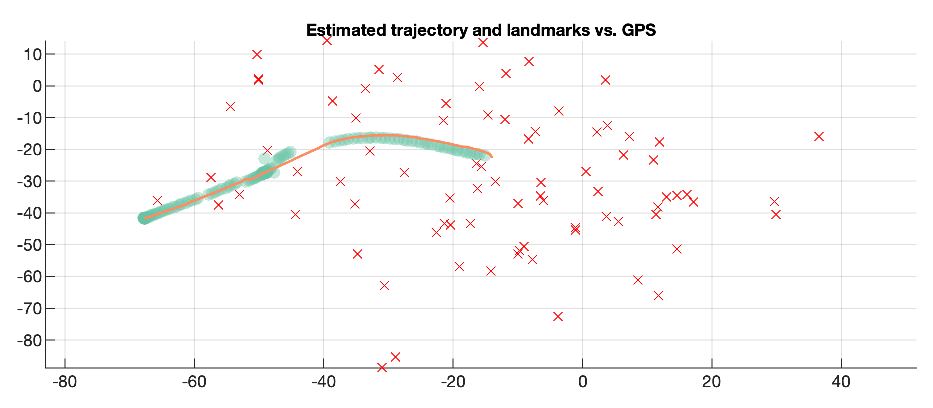
\includegraphics[width=0.6\linewidth]{figures/ga_2/real_trajectory.eps}
    \caption{}
    \label{fig:ga_2_real_trajectory}
\end{figure}

\begin{figure}[!htb]
    \centering
    \includegraphics[width=0.8\linewidth]{figures/ga_2/real_state.eps}
    \caption{}
    \label{fig:ga_2_real_state}
\end{figure}

\begin{figure}[!htb]
    \centering
    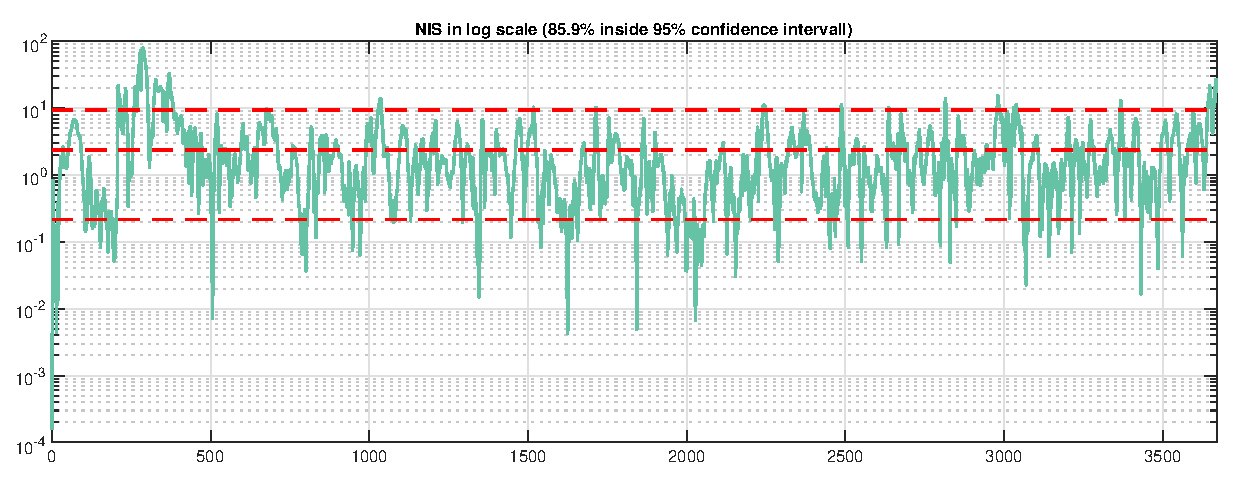
\includegraphics[width=0.8\linewidth]{figures/ga_2/real_consistency.eps}
    \caption{}
    \label{fig:ga_2_real_consistency}
\end{figure}

\begin{figure}[ht]
    \centering
	\begin{subfigure}[b]{0.45\textwidth}
		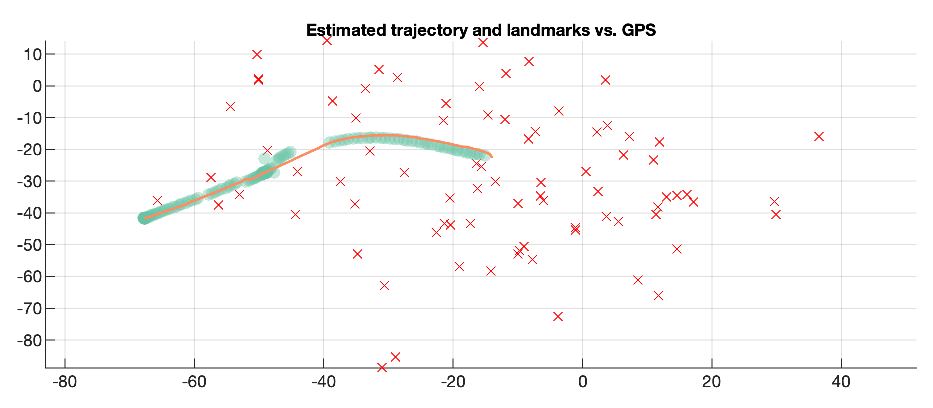
\includegraphics[width=\textwidth]{figures/ga_2/real_trajectory.eps}
    \caption{}
    \label{fig:ga_2_real_trajectory}
	\end{subfigure}%
       ~
	\begin{subfigure}[b]{0.45\textwidth}
		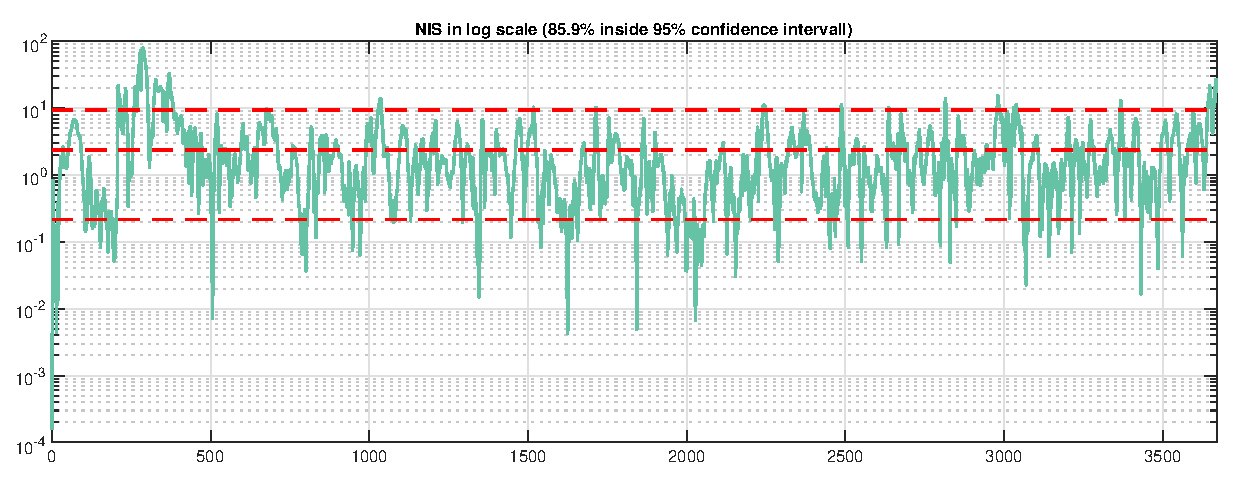
\includegraphics[width=\textwidth]{figures/ga_2/real_consistency.eps}
    \caption{}
    \label{fig:ga_2_real_consistency}
	\end{subfigure}
    \label{fig:ga_2_real_trajectory_consistency} 
\end{figure}